%% Autor: Björn Ritterbecks 
%% Letzte Aenderung: 15.06.2016 
\thisfloatsetup{%
  capbesidewidth=\marginparwidth}
\begin{figure}[htbp]
\vspace*{0.2cm}
\centering
%\sansmath
 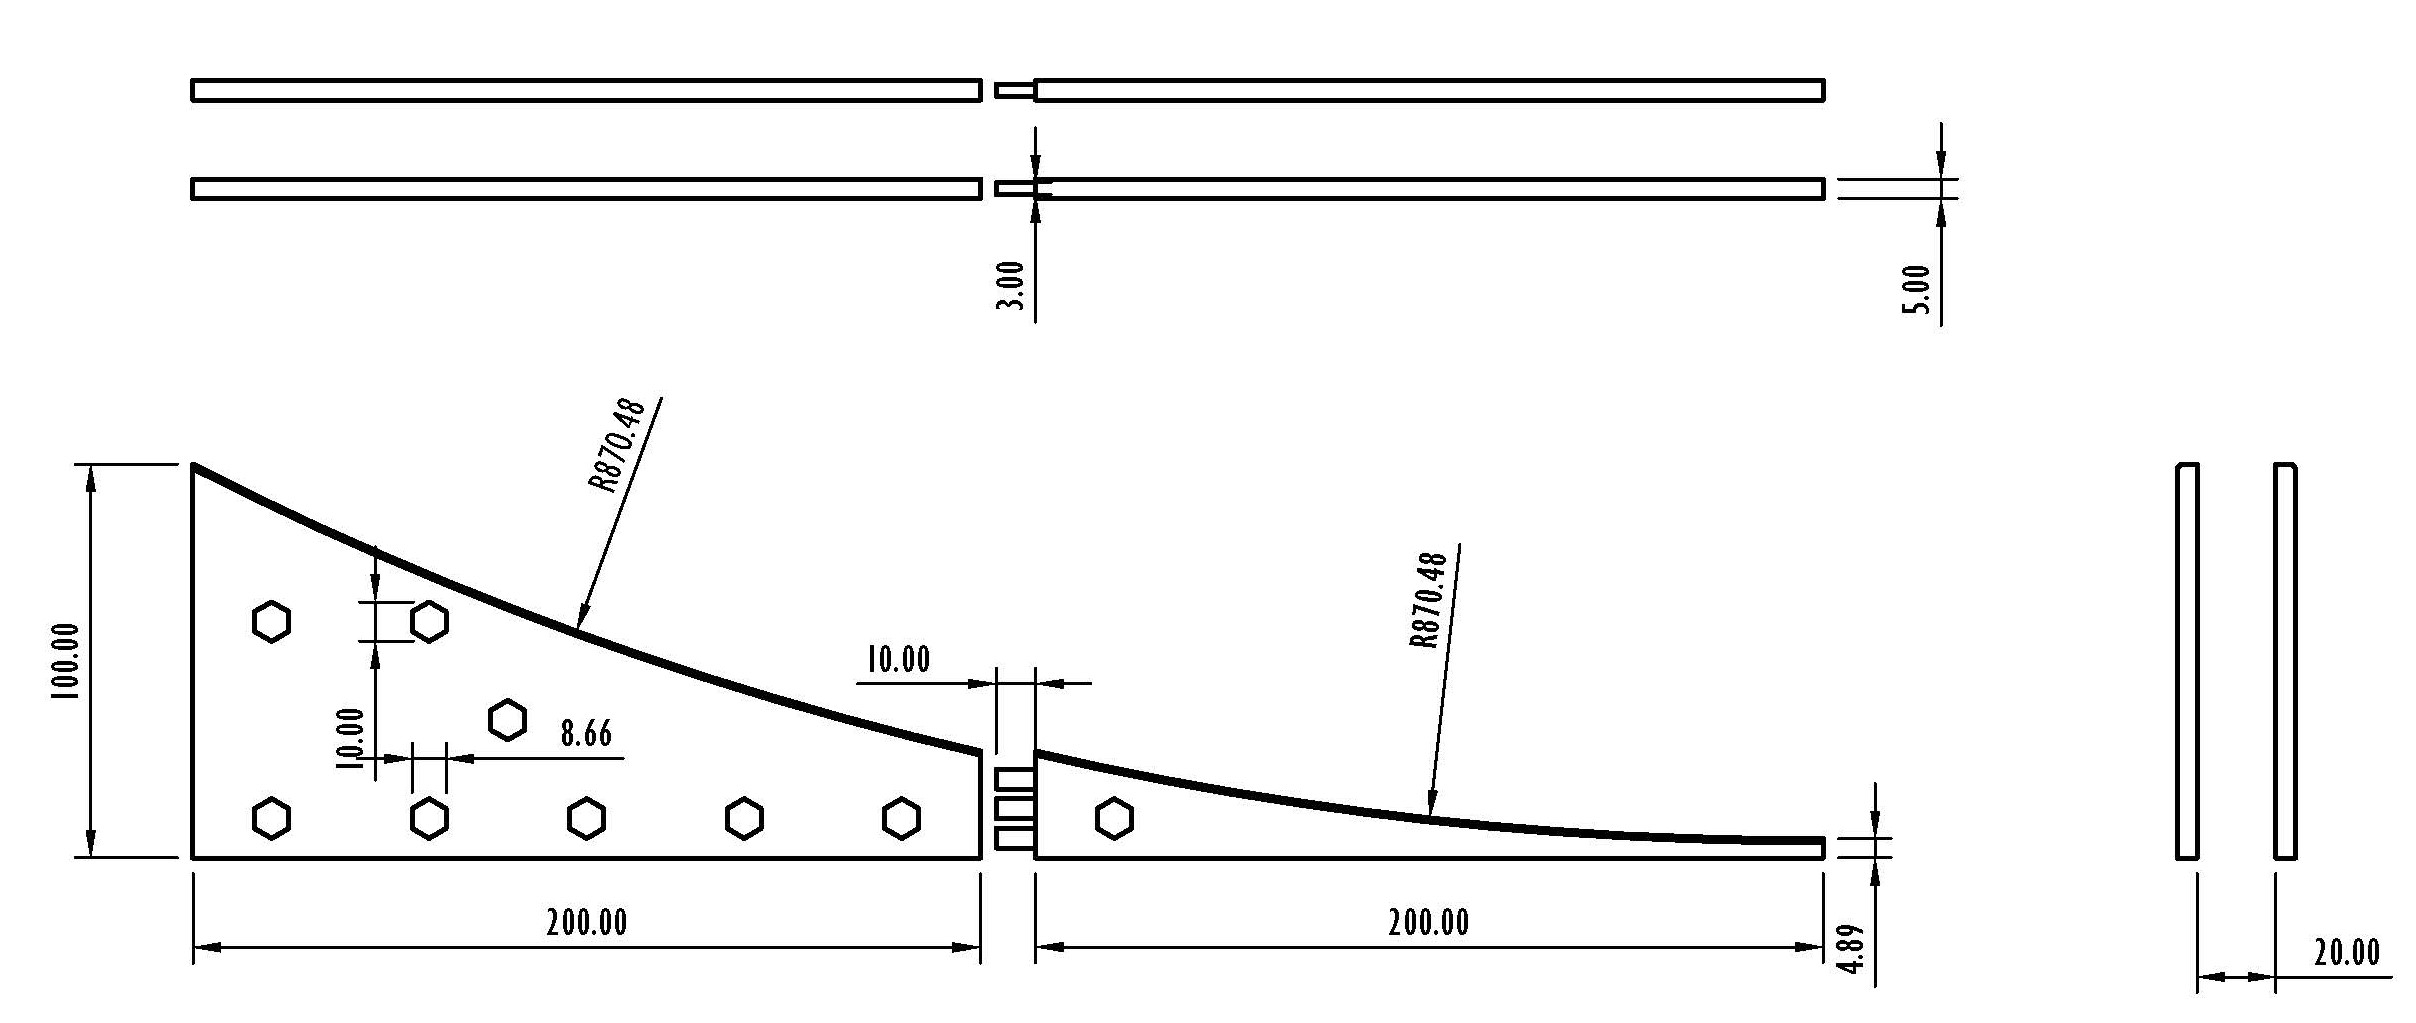
\includegraphics[width=0.99\textwidth]{images/rampedraw2.jpg}
  \caption[Technische Zeichnung der Beschleunigereinheit]{Zu sehen ist eine technische Zeichnung der geplanten Beschleunigereinheit, die auf einen 3D-Druck ausgelegt ist, jedoch mit leichten Anpassungen auch auf einer \textsw{CNC-Fräse} aus einer Stahlplatte mit Dicke $d=\SI{5}{\milli\metre}$ gefertigt werden kann. Die Rampe besitzt durch  die Aussparung eines Kreisbogens mit Radius $r=\SI{900}{\milli\metre}$ von $\SI{267.2}{\degree}$ bis $\SI{270}{\degree}$ einen nahezu waagerechten Auslauf.}
  \label{fig:rampedraw}
  \vspace{-0pt}
\end{figure}